\documentclass[1p]{elsarticle_modified}
%\bibliographystyle{elsarticle-num}

%\usepackage[colorlinks]{hyperref}
%\usepackage{abbrmath_seonhwa} %\Abb, \Ascr, \Acal ,\Abf, \Afrak
\usepackage{amsfonts}
\usepackage{amssymb}
\usepackage{amsmath}
\usepackage{amsthm}
\usepackage{scalefnt}
\usepackage{amsbsy}
\usepackage{kotex}
\usepackage{caption}
\usepackage{subfig}
\usepackage{color}
\usepackage{graphicx}
\usepackage{xcolor} %% white, black, red, green, blue, cyan, magenta, yellow
\usepackage{float}
\usepackage{setspace}
\usepackage{hyperref}

\usepackage{tikz}
\usetikzlibrary{arrows}

\usepackage{multirow}
\usepackage{array} % fixed length table
\usepackage{hhline}

%%%%%%%%%%%%%%%%%%%%%
\makeatletter
\renewcommand*\env@matrix[1][\arraystretch]{%
	\edef\arraystretch{#1}%
	\hskip -\arraycolsep
	\let\@ifnextchar\new@ifnextchar
	\array{*\c@MaxMatrixCols c}}
\makeatother %https://tex.stackexchange.com/questions/14071/how-can-i-increase-the-line-spacing-in-a-matrix
%%%%%%%%%%%%%%%

\usepackage[normalem]{ulem}

\newcommand{\msout}[1]{\ifmmode\text{\sout{\ensuremath{#1}}}\else\sout{#1}\fi}
%SOURCE: \msout is \stkout macro in https://tex.stackexchange.com/questions/20609/strikeout-in-math-mode

\newcommand{\cancel}[1]{
	\ifmmode
	{\color{red}\msout{#1}}
	\else
	{\color{red}\sout{#1}}
	\fi
}

\newcommand{\add}[1]{
	{\color{blue}\uwave{#1}}
}

\newcommand{\replace}[2]{
	\ifmmode
	{\color{red}\msout{#1}}{\color{blue}\uwave{#2}}
	\else
	{\color{red}\sout{#1}}{\color{blue}\uwave{#2}}
	\fi
}

\newcommand{\Sol}{\mathcal{S}} %segment
\newcommand{\D}{D} %diagram
\newcommand{\A}{\mathcal{A}} %arc


%%%%%%%%%%%%%%%%%%%%%%%%%%%%%5 test

\def\sl{\operatorname{\textup{SL}}(2,\Cbb)}
\def\psl{\operatorname{\textup{PSL}}(2,\Cbb)}
\def\quan{\mkern 1mu \triangleright \mkern 1mu}

\theoremstyle{definition}
\newtheorem{thm}{Theorem}[section]
\newtheorem{prop}[thm]{Proposition}
\newtheorem{lem}[thm]{Lemma}
\newtheorem{ques}[thm]{Question}
\newtheorem{cor}[thm]{Corollary}
\newtheorem{defn}[thm]{Definition}
\newtheorem{exam}[thm]{Example}
\newtheorem{rmk}[thm]{Remark}
\newtheorem{alg}[thm]{Algorithm}

\newcommand{\I}{\sqrt{-1}}
\begin{document}

%\begin{frontmatter}
%
%\title{Boundary parabolic representations of knots up to 8 crossings}
%
%%% Group authors per affiliation:
%\author{Yunhi Cho} 
%\address{Department of Mathematics, University of Seoul, Seoul, Korea}
%\ead{yhcho@uos.ac.kr}
%
%
%\author{Seonhwa Kim} %\fnref{s_kim}}
%\address{Center for Geometry and Physics, Institute for Basic Science, Pohang, 37673, Korea}
%\ead{ryeona17@ibs.re.kr}
%
%\author{Hyuk Kim}
%\address{Department of Mathematical Sciences, Seoul National University, Seoul 08826, Korea}
%\ead{hyukkim@snu.ac.kr}
%
%\author{Seokbeom Yoon}
%\address{Department of Mathematical Sciences, Seoul National University, Seoul, 08826,  Korea}
%\ead{sbyoon15@snu.ac.kr}
%
%\begin{abstract}
%We find all boundary parabolic representation of knots up to 8 crossings.
%
%\end{abstract}
%\begin{keyword}
%    \MSC[2010] 57M25 
%\end{keyword}
%
%\end{frontmatter}

%\linenumbers
%\tableofcontents
%
\newcommand\colored[1]{\textcolor{white}{\rule[-0.35ex]{0.8em}{1.4ex}}\kern-0.8em\color{red} #1}%
%\newcommand\colored[1]{\textcolor{white}{ #1}\kern-2.17ex	\textcolor{white}{ #1}\kern-1.81ex	\textcolor{white}{ #1}\kern-2.15ex\color{red}#1	}

{\Large $\underline{12n_{0852}~(K12n_{0852})}$}

\setlength{\tabcolsep}{10pt}
\renewcommand{\arraystretch}{1.6}
\vspace{1cm}\begin{tabular}{m{100pt}>{\centering\arraybackslash}m{274pt}}
\multirow{5}{120pt}{
	\centering
	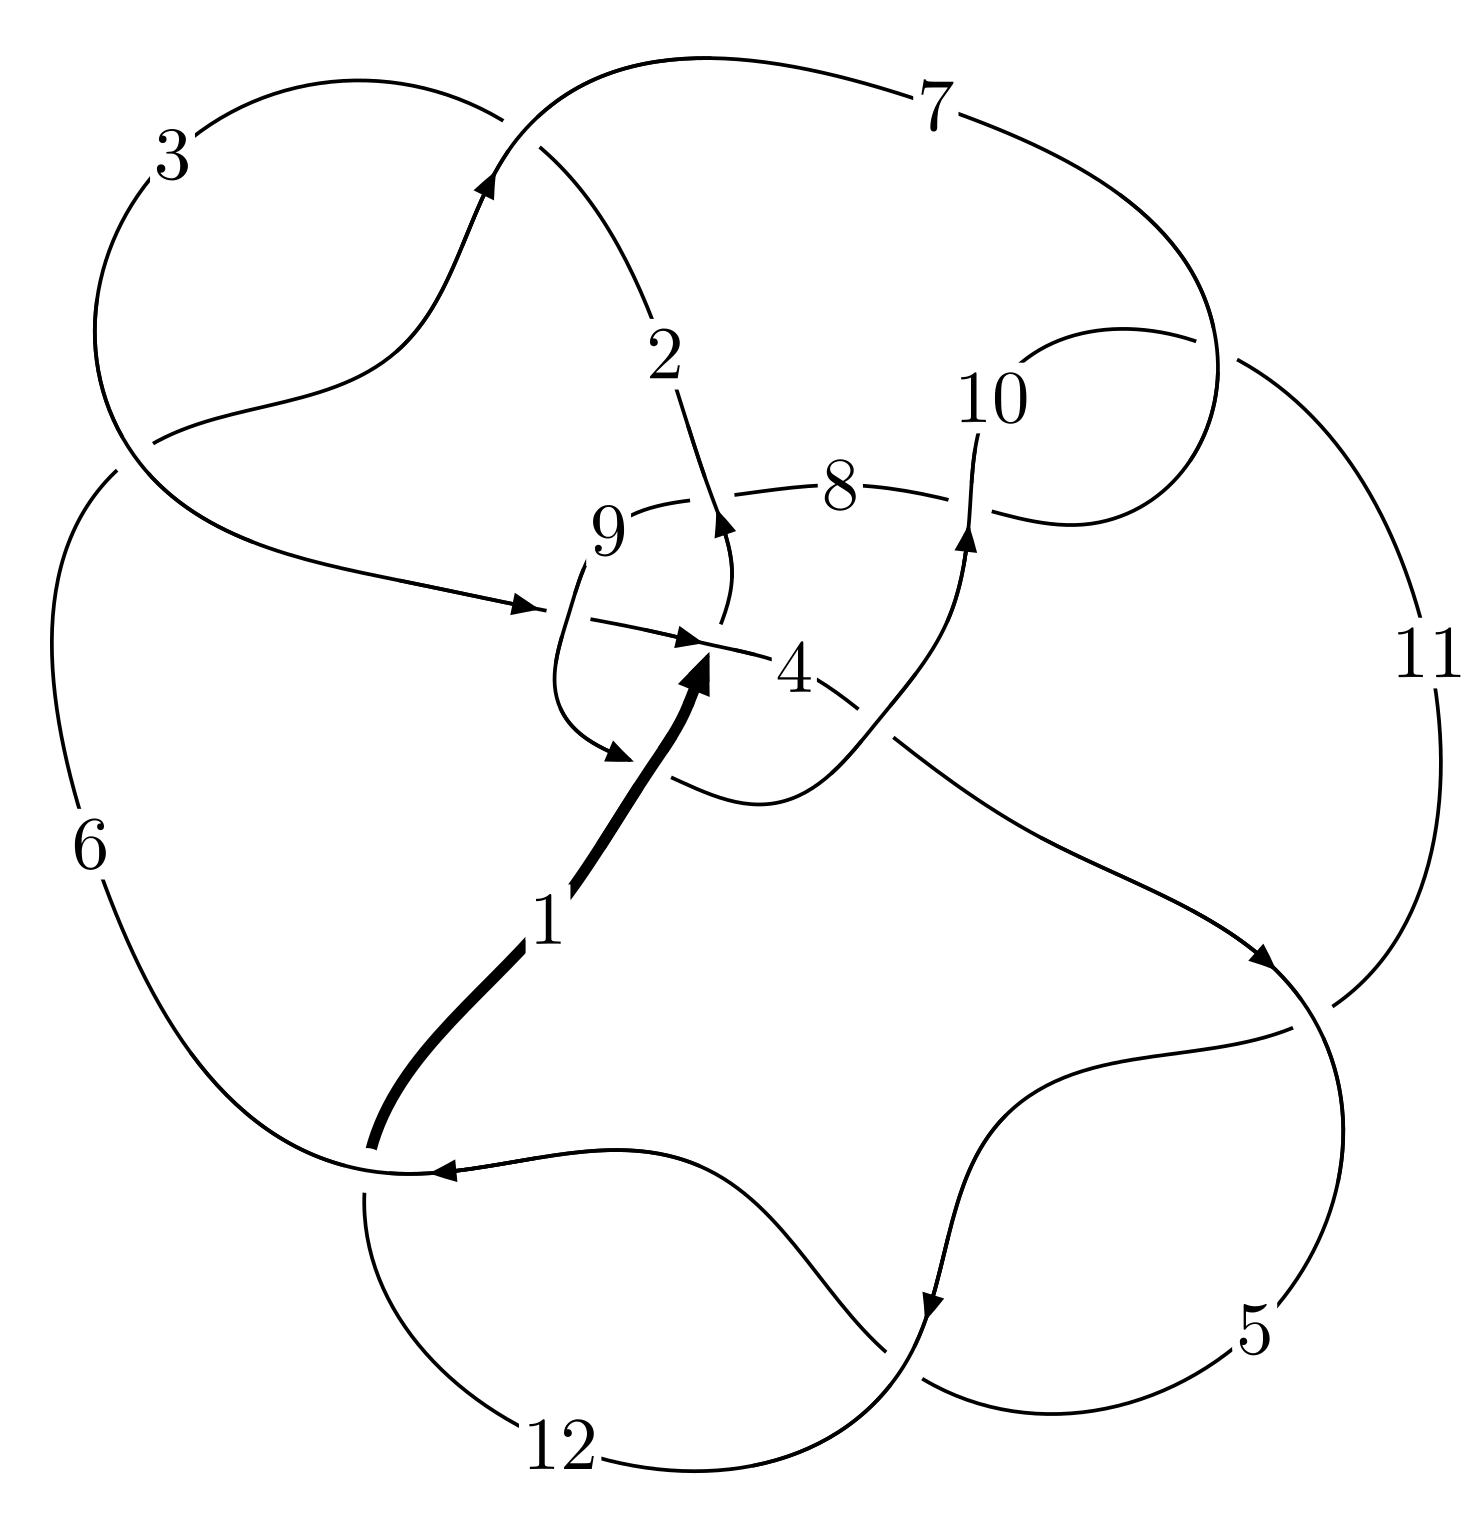
\includegraphics[width=112pt]{../../../GIT/diagram.site/Diagrams/png/2941_12n_0852.png}\\
\ \ \ A knot diagram\footnotemark}&
\allowdisplaybreaks
\textbf{Linearized knot diagam} \\
\cline{2-2}
 &
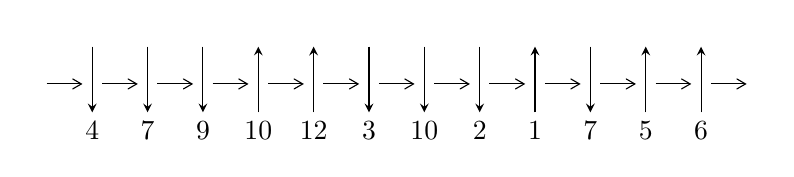
\begin{tikzpicture}[x=20pt, y=17pt]
	% nodes
	\node (C0) at (0, 0) {};
	\node (C1) at (1, 0) {};
	\node (C1U) at (1, +1) {};
	\node (C1D) at (1, -1) {4};

	\node (C2) at (2, 0) {};
	\node (C2U) at (2, +1) {};
	\node (C2D) at (2, -1) {7};

	\node (C3) at (3, 0) {};
	\node (C3U) at (3, +1) {};
	\node (C3D) at (3, -1) {9};

	\node (C4) at (4, 0) {};
	\node (C4U) at (4, +1) {};
	\node (C4D) at (4, -1) {10};

	\node (C5) at (5, 0) {};
	\node (C5U) at (5, +1) {};
	\node (C5D) at (5, -1) {12};

	\node (C6) at (6, 0) {};
	\node (C6U) at (6, +1) {};
	\node (C6D) at (6, -1) {3};

	\node (C7) at (7, 0) {};
	\node (C7U) at (7, +1) {};
	\node (C7D) at (7, -1) {10};

	\node (C8) at (8, 0) {};
	\node (C8U) at (8, +1) {};
	\node (C8D) at (8, -1) {2};

	\node (C9) at (9, 0) {};
	\node (C9U) at (9, +1) {};
	\node (C9D) at (9, -1) {1};

	\node (C10) at (10, 0) {};
	\node (C10U) at (10, +1) {};
	\node (C10D) at (10, -1) {7};

	\node (C11) at (11, 0) {};
	\node (C11U) at (11, +1) {};
	\node (C11D) at (11, -1) {5};

	\node (C12) at (12, 0) {};
	\node (C12U) at (12, +1) {};
	\node (C12D) at (12, -1) {6};
	\node (C13) at (13, 0) {};

	% arrows
	\draw[->,>={angle 60}]
	(C0) edge (C1) (C1) edge (C2) (C2) edge (C3) (C3) edge (C4) (C4) edge (C5) (C5) edge (C6) (C6) edge (C7) (C7) edge (C8) (C8) edge (C9) (C9) edge (C10) (C10) edge (C11) (C11) edge (C12) (C12) edge (C13) ;	\draw[->,>=stealth]
	(C1U) edge (C1D) (C2U) edge (C2D) (C3U) edge (C3D) (C4D) edge (C4U) (C5D) edge (C5U) (C6U) edge (C6D) (C7U) edge (C7D) (C8U) edge (C8D) (C9D) edge (C9U) (C10U) edge (C10D) (C11D) edge (C11U) (C12D) edge (C12U) ;
	\end{tikzpicture} \\
\hhline{~~} \\& 
\textbf{Solving Sequence} \\ \cline{2-2} 
 &
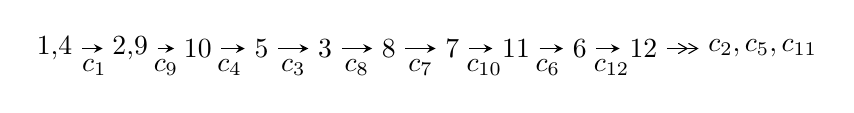
\begin{tikzpicture}[x=23pt, y=7pt]
	% node
	\node (A0) at (-1/8, 0) {1,4};
	\node (A1) at (17/16, 0) {2,9};
	\node (A2) at (17/8, 0) {10};
	\node (A3) at (25/8, 0) {5};
	\node (A4) at (33/8, 0) {3};
	\node (A5) at (41/8, 0) {8};
	\node (A6) at (49/8, 0) {7};
	\node (A7) at (57/8, 0) {11};
	\node (A8) at (65/8, 0) {6};
	\node (A9) at (73/8, 0) {12};
	\node (C1) at (1/2, -1) {$c_{1}$};
	\node (C2) at (13/8, -1) {$c_{9}$};
	\node (C3) at (21/8, -1) {$c_{4}$};
	\node (C4) at (29/8, -1) {$c_{3}$};
	\node (C5) at (37/8, -1) {$c_{8}$};
	\node (C6) at (45/8, -1) {$c_{7}$};
	\node (C7) at (53/8, -1) {$c_{10}$};
	\node (C8) at (61/8, -1) {$c_{6}$};
	\node (C9) at (69/8, -1) {$c_{12}$};
	\node (A10) at (11, 0) {$c_{2},c_{5},c_{11}$};

	% edge
	\draw[->,>=stealth]	
	(A0) edge (A1) (A1) edge (A2) (A2) edge (A3) (A3) edge (A4) (A4) edge (A5) (A5) edge (A6) (A6) edge (A7) (A7) edge (A8) (A8) edge (A9) ;
	\draw[->>,>={angle 60}]	
	(A9) edge (A10);
\end{tikzpicture} \\ 

\end{tabular} \\

\footnotetext{
The image of knot diagram is generated by the software ``\textbf{Draw programme}" developed by Andrew Bartholomew(\url{http://www.layer8.co.uk/maths/draw/index.htm\#Running-draw}), where we modified some parts for our purpose(\url{https://github.com/CATsTAILs/LinksPainter}).
}\phantom \\ \newline 
\centering \textbf{Ideals for irreducible components\footnotemark of $X_{\text{par}}$} 
 
\begin{align*}
I^u_{1}&=\langle 
3.07370\times10^{309} u^{88}+7.02933\times10^{309} u^{87}+\cdots+4.88148\times10^{305} b-4.73335\times10^{310},\\
\phantom{I^u_{1}}&\phantom{= \langle  }-5.19770\times10^{310} u^{88}-1.16472\times10^{311} u^{87}+\cdots+9.12837\times10^{307} a+6.31502\times10^{311},\\
\phantom{I^u_{1}}&\phantom{= \langle  }u^{89}+3 u^{88}+\cdots-128 u-11\rangle \\
I^u_{2}&=\langle 
5.39113\times10^{24} u^{26}-2.77278\times10^{25} u^{25}+\cdots+3.88238\times10^{24} b+3.65850\times10^{25},\\
\phantom{I^u_{2}}&\phantom{= \langle  }3.40177\times10^{25} u^{26}-1.13953\times10^{26} u^{25}+\cdots+3.88238\times10^{24} a+4.53762\times10^{25},\;u^{27}-4 u^{26}+\cdots+7 u-1\rangle \\
\\
\end{align*}
\raggedright * 2 irreducible components of $\dim_{\mathbb{C}}=0$, with total 116 representations.\\
\footnotetext{All coefficients of polynomials are rational numbers. But the coefficients are sometimes approximated in decimal forms when there is not enough margin.}
\newpage
\renewcommand{\arraystretch}{1}
\centering \section*{I. $I^u_{1}= \langle 3.07\times10^{309} u^{88}+7.03\times10^{309} u^{87}+\cdots+4.88\times10^{305} b-4.73\times10^{310},\;-5.20\times10^{310} u^{88}-1.16\times10^{311} u^{87}+\cdots+9.13\times10^{307} a+6.32\times10^{311},\;u^{89}+3 u^{88}+\cdots-128 u-11 \rangle$}
\flushleft \textbf{(i) Arc colorings}\\
\begin{tabular}{m{7pt} m{180pt} m{7pt} m{180pt} }
\flushright $a_{1}=$&$\begin{pmatrix}1\\0\end{pmatrix}$ \\
\flushright $a_{4}=$&$\begin{pmatrix}0\\u\end{pmatrix}$ \\
\flushright $a_{2}=$&$\begin{pmatrix}1\\u^2\end{pmatrix}$ \\
\flushright $a_{9}=$&$\begin{pmatrix}569.400 u^{88}+1275.94 u^{87}+\cdots-76010.6 u-6918.01\\-6296.66 u^{88}-14400.0 u^{87}+\cdots+992607. u+96965.4\end{pmatrix}$ \\
\flushright $a_{10}=$&$\begin{pmatrix}-5727.26 u^{88}-13124.0 u^{87}+\cdots+916597. u+90047.4\\-6296.66 u^{88}-14400.0 u^{87}+\cdots+992607. u+96965.4\end{pmatrix}$ \\
\flushright $a_{5}=$&$\begin{pmatrix}9085.14 u^{88}+21847.1 u^{87}+\cdots-1.67677\times10^{6} u-168656.\\3271.85 u^{88}+7597.71 u^{87}+\cdots-544620. u-53820.5\end{pmatrix}$ \\
\flushright $a_{3}=$&$\begin{pmatrix}5108.21 u^{88}+12633.7 u^{87}+\cdots-1.02025\times10^{6} u-103895.\\705.083 u^{88}+1615.68 u^{87}+\cdots-111892. u-10941.3\end{pmatrix}$ \\
\flushright $a_{8}=$&$\begin{pmatrix}-6026.68 u^{88}-13826.0 u^{87}+\cdots+965663. u+94802.3\\-9614.20 u^{88}-22011.9 u^{87}+\cdots+1.51990\times10^{6} u+148515.\end{pmatrix}$ \\
\flushright $a_{7}=$&$\begin{pmatrix}-3942.79 u^{88}-9158.68 u^{87}+\cdots+643604. u+62940.5\\-12173.0 u^{88}-28391.4 u^{87}+\cdots+2.03504\times10^{6} u+200771.\end{pmatrix}$ \\
\flushright $a_{11}=$&$\begin{pmatrix}-20489.4 u^{88}-47720.8 u^{87}+\cdots+3.42997\times10^{6} u+339274.\\-9470.05 u^{88}-21709.7 u^{87}+\cdots+1.49822\times10^{6} u+146332.\end{pmatrix}$ \\
\flushright $a_{6}=$&$\begin{pmatrix}7371.14 u^{88}+18256.7 u^{87}+\cdots-1.50139\times10^{6} u-154005.\\-3644.14 u^{88}-8508.11 u^{87}+\cdots+609864. u+60134.4\end{pmatrix}$ \\
\flushright $a_{12}=$&$\begin{pmatrix}-21862.8 u^{88}-52168.9 u^{87}+\cdots+3.95274\times10^{6} u+396541.\\-3836.25 u^{88}-8831.88 u^{87}+\cdots+618854. u+60764.8\end{pmatrix}$\\&\end{tabular}
\flushleft \textbf{(ii) Obstruction class $= -1$}\\~\\
\flushleft \textbf{(iii) Cusp Shapes $= 66908.2 u^{88}+158354. u^{87}+\cdots-1.16675\times10^{7} u-1.15911\times10^{6}$}\\~\\
\newpage\renewcommand{\arraystretch}{1}
\flushleft \textbf{(iv) u-Polynomials at the component}\newline \\
\begin{tabular}{m{50pt}|m{274pt}}
Crossings & \hspace{64pt}u-Polynomials at each crossing \\
\hline $$\begin{aligned}c_{1}\end{aligned}$$&$\begin{aligned}
&u^{89}-3 u^{88}+\cdots-128 u+11
\end{aligned}$\\
\hline $$\begin{aligned}c_{2},c_{6}\end{aligned}$$&$\begin{aligned}
&u^{89}- u^{88}+\cdots-2324 u+244
\end{aligned}$\\
\hline $$\begin{aligned}c_{3}\end{aligned}$$&$\begin{aligned}
&u^{89}+u^{88}+\cdots-35 u+1
\end{aligned}$\\
\hline $$\begin{aligned}c_{4}\end{aligned}$$&$\begin{aligned}
&u^{89}- u^{88}+\cdots-24352 u+16832
\end{aligned}$\\
\hline $$\begin{aligned}c_{5},c_{11},c_{12}\end{aligned}$$&$\begin{aligned}
&u^{89}-40 u^{87}+\cdots-525 u-299
\end{aligned}$\\
\hline $$\begin{aligned}c_{7},c_{10}\end{aligned}$$&$\begin{aligned}
&u^{89}+12 u^{88}+\cdots-33668 u-16181
\end{aligned}$\\
\hline $$\begin{aligned}c_{8}\end{aligned}$$&$\begin{aligned}
&u^{89}- u^{88}+\cdots-126958 u-15503
\end{aligned}$\\
\hline $$\begin{aligned}c_{9}\end{aligned}$$&$\begin{aligned}
&u^{89}-5 u^{88}+\cdots-25 u-1
\end{aligned}$\\
\hline
\end{tabular}\\~\\
\newpage\renewcommand{\arraystretch}{1}
\flushleft \textbf{(v) Riley Polynomials at the component}\newline \\
\begin{tabular}{m{50pt}|m{274pt}}
Crossings & \hspace{64pt}Riley Polynomials at each crossing \\
\hline $$\begin{aligned}c_{1}\end{aligned}$$&$\begin{aligned}
&y^{89}-17 y^{88}+\cdots+4372 y-121
\end{aligned}$\\
\hline $$\begin{aligned}c_{2},c_{6}\end{aligned}$$&$\begin{aligned}
&y^{89}+37 y^{88}+\cdots+79336 y-59536
\end{aligned}$\\
\hline $$\begin{aligned}c_{3}\end{aligned}$$&$\begin{aligned}
&y^{89}-5 y^{88}+\cdots+207 y-1
\end{aligned}$\\
\hline $$\begin{aligned}c_{4}\end{aligned}$$&$\begin{aligned}
&y^{89}+33 y^{88}+\cdots-15159981568 y-283316224
\end{aligned}$\\
\hline $$\begin{aligned}c_{5},c_{11},c_{12}\end{aligned}$$&$\begin{aligned}
&y^{89}-80 y^{88}+\cdots-4317613 y-89401
\end{aligned}$\\
\hline $$\begin{aligned}c_{7},c_{10}\end{aligned}$$&$\begin{aligned}
&y^{89}-70 y^{88}+\cdots+4270382884 y-261824761
\end{aligned}$\\
\hline $$\begin{aligned}c_{8}\end{aligned}$$&$\begin{aligned}
&y^{89}-29 y^{88}+\cdots-1482160124 y-240343009
\end{aligned}$\\
\hline $$\begin{aligned}c_{9}\end{aligned}$$&$\begin{aligned}
&y^{89}+5 y^{88}+\cdots+231 y-1
\end{aligned}$\\
\hline
\end{tabular}\\~\\
\newpage\flushleft \textbf{(vi) Complex Volumes and Cusp Shapes}
$$\begin{array}{c|c|c}  
\text{Solutions to }I^u_{1}& \I (\text{vol} + \sqrt{-1}CS) & \text{Cusp shape}\\
 \hline 
\begin{aligned}
u &= -0.993067 + 0.127078 I \\
a &= \phantom{-}0.200540 + 0.455929 I \\
b &= -0.33540 - 1.39904 I\end{aligned}
 & \phantom{-}3.20078 - 1.20884 I & \phantom{-0.000000 } 0 \\ \hline\begin{aligned}
u &= -0.993067 - 0.127078 I \\
a &= \phantom{-}0.200540 - 0.455929 I \\
b &= -0.33540 + 1.39904 I\end{aligned}
 & \phantom{-}3.20078 + 1.20884 I & \phantom{-0.000000 } 0 \\ \hline\begin{aligned}
u &= \phantom{-}0.764241 + 0.676726 I \\
a &= -0.947281 - 0.895205 I \\
b &= \phantom{-}0.340493 - 0.833126 I\end{aligned}
 & -0.57886 - 1.51432 I & \phantom{-0.000000 } 0 \\ \hline\begin{aligned}
u &= \phantom{-}0.764241 - 0.676726 I \\
a &= -0.947281 + 0.895205 I \\
b &= \phantom{-}0.340493 + 0.833126 I\end{aligned}
 & -0.57886 + 1.51432 I & \phantom{-0.000000 } 0 \\ \hline\begin{aligned}
u &= -0.760022 + 0.609380 I \\
a &= -1.39086 + 0.41043 I \\
b &= \phantom{-}0.928173 + 1.010740 I\end{aligned}
 & \phantom{-}1.56089 + 4.86458 I & \phantom{-0.000000 } 0 \\ \hline\begin{aligned}
u &= -0.760022 - 0.609380 I \\
a &= -1.39086 - 0.41043 I \\
b &= \phantom{-}0.928173 - 1.010740 I\end{aligned}
 & \phantom{-}1.56089 - 4.86458 I & \phantom{-0.000000 } 0 \\ \hline\begin{aligned}
u &= \phantom{-}0.689207 + 0.762844 I \\
a &= -0.728813 + 0.323818 I \\
b &= \phantom{-}1.097610 - 0.099960 I\end{aligned}
 & -0.45328 - 4.13288 I & \phantom{-0.000000 } 0 \\ \hline\begin{aligned}
u &= \phantom{-}0.689207 - 0.762844 I \\
a &= -0.728813 - 0.323818 I \\
b &= \phantom{-}1.097610 + 0.099960 I\end{aligned}
 & -0.45328 + 4.13288 I & \phantom{-0.000000 } 0 \\ \hline\begin{aligned}
u &= \phantom{-}1.005520 + 0.290922 I \\
a &= \phantom{-}0.818301 - 0.419258 I \\
b &= -0.017694 - 0.228854 I\end{aligned}
 & -2.29896 - 0.81375 I & \phantom{-0.000000 } 0 \\ \hline\begin{aligned}
u &= \phantom{-}1.005520 - 0.290922 I \\
a &= \phantom{-}0.818301 + 0.419258 I \\
b &= -0.017694 + 0.228854 I\end{aligned}
 & -2.29896 + 0.81375 I & \phantom{-0.000000 } 0\\
 \hline 
 \end{array}$$\newpage$$\begin{array}{c|c|c}  
\text{Solutions to }I^u_{1}& \I (\text{vol} + \sqrt{-1}CS) & \text{Cusp shape}\\
 \hline 
\begin{aligned}
u &= \phantom{-}0.683719 + 0.823293 I \\
a &= -0.798187 + 0.260059 I \\
b &= \phantom{-}0.779052 - 0.834217 I\end{aligned}
 & \phantom{-}0.04254 - 3.77924 I & \phantom{-0.000000 } 0 \\ \hline\begin{aligned}
u &= \phantom{-}0.683719 - 0.823293 I \\
a &= -0.798187 - 0.260059 I \\
b &= \phantom{-}0.779052 + 0.834217 I\end{aligned}
 & \phantom{-}0.04254 + 3.77924 I & \phantom{-0.000000 } 0 \\ \hline\begin{aligned}
u &= \phantom{-}0.898322 + 0.057751 I \\
a &= -1.47888 - 0.45299 I \\
b &= -0.394720 - 0.110803 I\end{aligned}
 & \phantom{-}4.30044 + 0.66708 I & \phantom{-0.000000 } 0 \\ \hline\begin{aligned}
u &= \phantom{-}0.898322 - 0.057751 I \\
a &= -1.47888 + 0.45299 I \\
b &= -0.394720 + 0.110803 I\end{aligned}
 & \phantom{-}4.30044 - 0.66708 I & \phantom{-0.000000 } 0 \\ \hline\begin{aligned}
u &= \phantom{-}0.669022 + 0.568571 I \\
a &= \phantom{-}1.55704 - 0.05911 I \\
b &= -1.49947 + 0.46973 I\end{aligned}
 & \phantom{-}5.72482 - 2.22060 I & \phantom{-0.000000 } 0 \\ \hline\begin{aligned}
u &= \phantom{-}0.669022 - 0.568571 I \\
a &= \phantom{-}1.55704 + 0.05911 I \\
b &= -1.49947 - 0.46973 I\end{aligned}
 & \phantom{-}5.72482 + 2.22060 I & \phantom{-0.000000 } 0 \\ \hline\begin{aligned}
u &= -0.902065 + 0.669900 I \\
a &= \phantom{-}1.382100 - 0.221188 I \\
b &= -1.14788 - 0.96298 I\end{aligned}
 & \phantom{-}5.44061 + 8.85234 I & \phantom{-0.000000 } 0 \\ \hline\begin{aligned}
u &= -0.902065 - 0.669900 I \\
a &= \phantom{-}1.382100 + 0.221188 I \\
b &= -1.14788 + 0.96298 I\end{aligned}
 & \phantom{-}5.44061 - 8.85234 I & \phantom{-0.000000 } 0 \\ \hline\begin{aligned}
u &= \phantom{-}0.995812 + 0.570446 I \\
a &= -0.155902 + 0.043006 I \\
b &= \phantom{-}0.301459 + 0.908339 I\end{aligned}
 & -1.22561 - 3.72621 I & \phantom{-0.000000 } 0 \\ \hline\begin{aligned}
u &= \phantom{-}0.995812 - 0.570446 I \\
a &= -0.155902 - 0.043006 I \\
b &= \phantom{-}0.301459 - 0.908339 I\end{aligned}
 & -1.22561 + 3.72621 I & \phantom{-0.000000 } 0\\
 \hline 
 \end{array}$$\newpage$$\begin{array}{c|c|c}  
\text{Solutions to }I^u_{1}& \I (\text{vol} + \sqrt{-1}CS) & \text{Cusp shape}\\
 \hline 
\begin{aligned}
u &= \phantom{-}0.705441 + 0.470348 I \\
a &= \phantom{-}0.980226 - 0.082282 I \\
b &= -0.273554 + 0.437450 I\end{aligned}
 & -1.23728 - 0.76406 I & \phantom{-0.000000 } 0 \\ \hline\begin{aligned}
u &= \phantom{-}0.705441 - 0.470348 I \\
a &= \phantom{-}0.980226 + 0.082282 I \\
b &= -0.273554 - 0.437450 I\end{aligned}
 & -1.23728 + 0.76406 I & \phantom{-0.000000 } 0 \\ \hline\begin{aligned}
u &= \phantom{-}0.684498 + 0.448987 I \\
a &= -0.19969 + 2.02237 I \\
b &= -0.360630 + 0.502464 I\end{aligned}
 & -3.27660 - 4.26157 I & \phantom{-0.000000 } 0 \\ \hline\begin{aligned}
u &= \phantom{-}0.684498 - 0.448987 I \\
a &= -0.19969 - 2.02237 I \\
b &= -0.360630 - 0.502464 I\end{aligned}
 & -3.27660 + 4.26157 I & \phantom{-0.000000 } 0 \\ \hline\begin{aligned}
u &= -0.552981 + 1.083490 I \\
a &= -1.42961 - 0.56881 I \\
b &= \phantom{-}0.560860 + 0.860648 I\end{aligned}
 & \phantom{-}6.74974 + 6.19688 I & \phantom{-0.000000 } 0 \\ \hline\begin{aligned}
u &= -0.552981 - 1.083490 I \\
a &= -1.42961 + 0.56881 I \\
b &= \phantom{-}0.560860 - 0.860648 I\end{aligned}
 & \phantom{-}6.74974 - 6.19688 I & \phantom{-0.000000 } 0 \\ \hline\begin{aligned}
u &= -0.450193 + 0.633301 I \\
a &= -0.478689 + 0.401501 I \\
b &= \phantom{-}0.734409 + 0.456658 I\end{aligned}
 & \phantom{-}1.29822 + 1.05454 I & \phantom{-0.000000 } 0 \\ \hline\begin{aligned}
u &= -0.450193 - 0.633301 I \\
a &= -0.478689 - 0.401501 I \\
b &= \phantom{-}0.734409 - 0.456658 I\end{aligned}
 & \phantom{-}1.29822 - 1.05454 I & \phantom{-0.000000 } 0 \\ \hline\begin{aligned}
u &= -0.743607 + 0.209729 I \\
a &= \phantom{-}0.31095 + 2.56899 I \\
b &= \phantom{-}0.236058 + 0.953099 I\end{aligned}
 & \phantom{-}1.43846 - 5.32495 I & \phantom{-0.000000 } 0 \\ \hline\begin{aligned}
u &= -0.743607 - 0.209729 I \\
a &= \phantom{-}0.31095 - 2.56899 I \\
b &= \phantom{-}0.236058 - 0.953099 I\end{aligned}
 & \phantom{-}1.43846 + 5.32495 I & \phantom{-0.000000 } 0\\
 \hline 
 \end{array}$$\newpage$$\begin{array}{c|c|c}  
\text{Solutions to }I^u_{1}& \I (\text{vol} + \sqrt{-1}CS) & \text{Cusp shape}\\
 \hline 
\begin{aligned}
u &= -0.501394 + 0.585172 I \\
a &= \phantom{-}2.05602 - 0.82578 I \\
b &= -0.736196 - 0.962460 I\end{aligned}
 & \phantom{-}6.03500 + 1.36427 I & \phantom{-0.000000 } 0 \\ \hline\begin{aligned}
u &= -0.501394 - 0.585172 I \\
a &= \phantom{-}2.05602 + 0.82578 I \\
b &= -0.736196 + 0.962460 I\end{aligned}
 & \phantom{-}6.03500 - 1.36427 I & \phantom{-0.000000 } 0 \\ \hline\begin{aligned}
u &= \phantom{-}0.670311 + 0.380079 I \\
a &= \phantom{-}0.999831 - 0.186322 I \\
b &= -1.63239 - 0.59106 I\end{aligned}
 & -3.33787 + 1.07323 I & \phantom{-0.000000 } 0 \\ \hline\begin{aligned}
u &= \phantom{-}0.670311 - 0.380079 I \\
a &= \phantom{-}0.999831 + 0.186322 I \\
b &= -1.63239 + 0.59106 I\end{aligned}
 & -3.33787 - 1.07323 I & \phantom{-0.000000 } 0 \\ \hline\begin{aligned}
u &= -0.767264\phantom{ +0.000000I} \\
a &= -1.97006\phantom{ +0.000000I} \\
b &= \phantom{-}0.928015\phantom{ +0.000000I}\end{aligned}
 & -4.39996\phantom{ +0.000000I} & \phantom{-0.000000 } 0 \\ \hline\begin{aligned}
u &= -0.572087 + 0.457673 I \\
a &= -0.839051 + 0.284723 I \\
b &= \phantom{-}1.69990 - 1.54093 I\end{aligned}
 & \phantom{-}2.29718 + 7.94648 I & \phantom{-0.000000 } 0 \\ \hline\begin{aligned}
u &= -0.572087 - 0.457673 I \\
a &= -0.839051 - 0.284723 I \\
b &= \phantom{-}1.69990 + 1.54093 I\end{aligned}
 & \phantom{-}2.29718 - 7.94648 I & \phantom{-0.000000 } 0 \\ \hline\begin{aligned}
u &= -0.932679 + 0.881057 I \\
a &= -1.105010 + 0.476206 I \\
b &= \phantom{-}0.968417 + 0.207288 I\end{aligned}
 & \phantom{-}9.26732 + 3.26395 I & \phantom{-0.000000 } 0 \\ \hline\begin{aligned}
u &= -0.932679 - 0.881057 I \\
a &= -1.105010 - 0.476206 I \\
b &= \phantom{-}0.968417 - 0.207288 I\end{aligned}
 & \phantom{-}9.26732 - 3.26395 I & \phantom{-0.000000 } 0 \\ \hline\begin{aligned}
u &= \phantom{-}0.708618 + 0.099564 I \\
a &= -1.371210 + 0.072508 I \\
b &= \phantom{-}1.76000 + 0.96153 I\end{aligned}
 & \phantom{-}1.07016 + 5.85705 I & \phantom{-0.000000 } 0\\
 \hline 
 \end{array}$$\newpage$$\begin{array}{c|c|c}  
\text{Solutions to }I^u_{1}& \I (\text{vol} + \sqrt{-1}CS) & \text{Cusp shape}\\
 \hline 
\begin{aligned}
u &= \phantom{-}0.708618 - 0.099564 I \\
a &= -1.371210 - 0.072508 I \\
b &= \phantom{-}1.76000 - 0.96153 I\end{aligned}
 & \phantom{-}1.07016 - 5.85705 I & \phantom{-0.000000 } 0 \\ \hline\begin{aligned}
u &= \phantom{-}0.604944 + 1.134220 I \\
a &= \phantom{-}0.701078 - 0.313258 I \\
b &= -1.25751 + 1.36163 I\end{aligned}
 & \phantom{-}8.06380 - 5.92574 I & \phantom{-0.000000 } 0 \\ \hline\begin{aligned}
u &= \phantom{-}0.604944 - 1.134220 I \\
a &= \phantom{-}0.701078 + 0.313258 I \\
b &= -1.25751 - 1.36163 I\end{aligned}
 & \phantom{-}8.06380 + 5.92574 I & \phantom{-0.000000 } 0 \\ \hline\begin{aligned}
u &= -0.803682 + 1.013040 I \\
a &= \phantom{-}1.159370 + 0.058891 I \\
b &= -0.659826 - 0.594923 I\end{aligned}
 & \phantom{-}3.75873 + 4.16261 I & \phantom{-0.000000 } 0 \\ \hline\begin{aligned}
u &= -0.803682 - 1.013040 I \\
a &= \phantom{-}1.159370 - 0.058891 I \\
b &= -0.659826 + 0.594923 I\end{aligned}
 & \phantom{-}3.75873 - 4.16261 I & \phantom{-0.000000 } 0 \\ \hline\begin{aligned}
u &= -0.680676 + 0.139986 I \\
a &= -1.03899 - 1.91698 I \\
b &= \phantom{-}0.055904 - 0.875204 I\end{aligned}
 & -4.56973 - 1.77199 I & \phantom{-0.000000 } 0 \\ \hline\begin{aligned}
u &= -0.680676 - 0.139986 I \\
a &= -1.03899 + 1.91698 I \\
b &= \phantom{-}0.055904 + 0.875204 I\end{aligned}
 & -4.56973 + 1.77199 I & \phantom{-0.000000 } 0 \\ \hline\begin{aligned}
u &= -0.674606 + 0.006235 I \\
a &= \phantom{-}0.434040 + 0.302717 I \\
b &= \phantom{-}0.358213 - 0.830103 I\end{aligned}
 & \phantom{-}1.09369 - 1.53017 I & \phantom{-0.000000 } 0 \\ \hline\begin{aligned}
u &= -0.674606 - 0.006235 I \\
a &= \phantom{-}0.434040 - 0.302717 I \\
b &= \phantom{-}0.358213 + 0.830103 I\end{aligned}
 & \phantom{-}1.09369 + 1.53017 I & \phantom{-0.000000 } 0 \\ \hline\begin{aligned}
u &= \phantom{-}0.568383 + 0.358844 I \\
a &= \phantom{-}1.02786 - 3.41911 I \\
b &= \phantom{-}0.469023 - 0.398181 I\end{aligned}
 & \phantom{-}1.82604 - 7.70258 I & \phantom{-0.000000 } 0\\
 \hline 
 \end{array}$$\newpage$$\begin{array}{c|c|c}  
\text{Solutions to }I^u_{1}& \I (\text{vol} + \sqrt{-1}CS) & \text{Cusp shape}\\
 \hline 
\begin{aligned}
u &= \phantom{-}0.568383 - 0.358844 I \\
a &= \phantom{-}1.02786 + 3.41911 I \\
b &= \phantom{-}0.469023 + 0.398181 I\end{aligned}
 & \phantom{-}1.82604 + 7.70258 I & \phantom{-0.000000 } 0 \\ \hline\begin{aligned}
u &= -0.656994 + 0.114545 I \\
a &= \phantom{-}0.196690 + 0.824596 I \\
b &= -0.02354 + 1.55734 I\end{aligned}
 & -3.92764 + 3.06811 I & \phantom{-0.000000 } 0 \\ \hline\begin{aligned}
u &= -0.656994 - 0.114545 I \\
a &= \phantom{-}0.196690 - 0.824596 I \\
b &= -0.02354 - 1.55734 I\end{aligned}
 & -3.92764 - 3.06811 I & \phantom{-0.000000 } 0 \\ \hline\begin{aligned}
u &= -0.959202 + 0.973290 I \\
a &= \phantom{-}0.630885 - 0.361979 I \\
b &= -1.39767 - 0.66471 I\end{aligned}
 & \phantom{-}10.28100 + 3.55115 I & \phantom{-0.000000 } 0 \\ \hline\begin{aligned}
u &= -0.959202 - 0.973290 I \\
a &= \phantom{-}0.630885 + 0.361979 I \\
b &= -1.39767 + 0.66471 I\end{aligned}
 & \phantom{-}10.28100 - 3.55115 I & \phantom{-0.000000 } 0 \\ \hline\begin{aligned}
u &= \phantom{-}0.354566 + 0.522064 I \\
a &= -1.69747 + 0.60020 I \\
b &= \phantom{-}1.117580 - 0.802866 I\end{aligned}
 & \phantom{-}1.79991 - 2.57496 I & \phantom{-0.000000 } 0 \\ \hline\begin{aligned}
u &= \phantom{-}0.354566 - 0.522064 I \\
a &= -1.69747 - 0.60020 I \\
b &= \phantom{-}1.117580 + 0.802866 I\end{aligned}
 & \phantom{-}1.79991 + 2.57496 I & \phantom{-0.000000 } 0 \\ \hline\begin{aligned}
u &= -0.579721 + 0.197706 I \\
a &= \phantom{-}0.646250 + 0.200700 I \\
b &= -0.90475 + 1.75982 I\end{aligned}
 & -4.14081 + 3.12659 I & \phantom{-0.000000 } 0 \\ \hline\begin{aligned}
u &= -0.579721 - 0.197706 I \\
a &= \phantom{-}0.646250 - 0.200700 I \\
b &= -0.90475 - 1.75982 I\end{aligned}
 & -4.14081 - 3.12659 I & \phantom{-0.000000 } 0 \\ \hline\begin{aligned}
u &= -0.247717 + 0.536375 I \\
a &= \phantom{-}0.69213 - 1.98581 I \\
b &= -0.691359 + 0.853223 I\end{aligned}
 & \phantom{-}6.36140 - 4.27453 I & \phantom{-0.000000 } 0\\
 \hline 
 \end{array}$$\newpage$$\begin{array}{c|c|c}  
\text{Solutions to }I^u_{1}& \I (\text{vol} + \sqrt{-1}CS) & \text{Cusp shape}\\
 \hline 
\begin{aligned}
u &= -0.247717 - 0.536375 I \\
a &= \phantom{-}0.69213 + 1.98581 I \\
b &= -0.691359 - 0.853223 I\end{aligned}
 & \phantom{-}6.36140 + 4.27453 I & \phantom{-0.000000 } 0 \\ \hline\begin{aligned}
u &= -0.575286\phantom{ +0.000000I} \\
a &= \phantom{-}4.34625\phantom{ +0.000000I} \\
b &= -0.0626997\phantom{ +0.000000I}\end{aligned}
 & -3.56473\phantom{ +0.000000I} & -23.9990\phantom{ +0.000000I} \\ \hline\begin{aligned}
u &= -1.17929 + 0.89101 I \\
a &= -0.822428 + 0.145424 I \\
b &= \phantom{-}1.15916 + 0.99640 I\end{aligned}
 & -1.24110 + 5.87258 I & \phantom{-0.000000 } 0 \\ \hline\begin{aligned}
u &= -1.17929 - 0.89101 I \\
a &= -0.822428 - 0.145424 I \\
b &= \phantom{-}1.15916 - 0.99640 I\end{aligned}
 & -1.24110 - 5.87258 I & \phantom{-0.000000 } 0 \\ \hline\begin{aligned}
u &= \phantom{-}0.24869 + 1.46137 I \\
a &= -0.453006 - 0.032139 I \\
b &= \phantom{-}0.673115 + 0.230690 I\end{aligned}
 & \phantom{-}1.42043 + 1.69576 I & \phantom{-0.000000 } 0 \\ \hline\begin{aligned}
u &= \phantom{-}0.24869 - 1.46137 I \\
a &= -0.453006 + 0.032139 I \\
b &= \phantom{-}0.673115 - 0.230690 I\end{aligned}
 & \phantom{-}1.42043 - 1.69576 I & \phantom{-0.000000 } 0 \\ \hline\begin{aligned}
u &= \phantom{-}1.20458 + 0.89965 I \\
a &= -1.003570 - 0.249439 I \\
b &= \phantom{-}0.933751 - 0.927723 I\end{aligned}
 & -0.82254 - 9.48836 I & \phantom{-0.000000 } 0 \\ \hline\begin{aligned}
u &= \phantom{-}1.20458 - 0.89965 I \\
a &= -1.003570 + 0.249439 I \\
b &= \phantom{-}0.933751 + 0.927723 I\end{aligned}
 & -0.82254 + 9.48836 I & \phantom{-0.000000 } 0 \\ \hline\begin{aligned}
u &= \phantom{-}1.17338 + 0.96189 I \\
a &= -0.864496 + 0.237008 I \\
b &= \phantom{-}0.61188 - 1.29209 I\end{aligned}
 & -2.32543 - 2.20605 I & \phantom{-0.000000 } 0 \\ \hline\begin{aligned}
u &= \phantom{-}1.17338 - 0.96189 I \\
a &= -0.864496 - 0.237008 I \\
b &= \phantom{-}0.61188 + 1.29209 I\end{aligned}
 & -2.32543 + 2.20605 I & \phantom{-0.000000 } 0\\
 \hline 
 \end{array}$$\newpage$$\begin{array}{c|c|c}  
\text{Solutions to }I^u_{1}& \I (\text{vol} + \sqrt{-1}CS) & \text{Cusp shape}\\
 \hline 
\begin{aligned}
u &= -1.19863 + 0.94740 I \\
a &= \phantom{-}0.967686 - 0.088945 I \\
b &= -1.12242 - 1.12580 I\end{aligned}
 & -3.70513 + 12.22050 I & \phantom{-0.000000 } 0 \\ \hline\begin{aligned}
u &= -1.19863 - 0.94740 I \\
a &= \phantom{-}0.967686 + 0.088945 I \\
b &= -1.12242 + 1.12580 I\end{aligned}
 & -3.70513 - 12.22050 I & \phantom{-0.000000 } 0 \\ \hline\begin{aligned}
u &= -1.18143 + 0.97516 I \\
a &= -1.098600 + 0.099827 I \\
b &= \phantom{-}1.14372 + 1.21653 I\end{aligned}
 & \phantom{-}1.8734 + 17.6191 I & \phantom{-0.000000 } 0 \\ \hline\begin{aligned}
u &= -1.18143 - 0.97516 I \\
a &= -1.098600 - 0.099827 I \\
b &= \phantom{-}1.14372 - 1.21653 I\end{aligned}
 & \phantom{-}1.8734 - 17.6191 I & \phantom{-0.000000 } 0 \\ \hline\begin{aligned}
u &= \phantom{-}1.22128 + 0.94280 I \\
a &= \phantom{-}0.898932 + 0.015878 I \\
b &= -0.762082 + 1.059560 I\end{aligned}
 & -5.54989 - 5.71430 I & \phantom{-0.000000 } 0 \\ \hline\begin{aligned}
u &= \phantom{-}1.22128 - 0.94280 I \\
a &= \phantom{-}0.898932 - 0.015878 I \\
b &= -0.762082 - 1.059560 I\end{aligned}
 & -5.54989 + 5.71430 I & \phantom{-0.000000 } 0 \\ \hline\begin{aligned}
u &= \phantom{-}1.10608 + 1.18820 I \\
a &= \phantom{-}0.588583 - 0.496668 I \\
b &= -0.111755 + 1.185780 I\end{aligned}
 & -1.62538 - 6.04479 I & \phantom{-0.000000 } 0 \\ \hline\begin{aligned}
u &= \phantom{-}1.10608 - 1.18820 I \\
a &= \phantom{-}0.588583 + 0.496668 I \\
b &= -0.111755 - 1.185780 I\end{aligned}
 & -1.62538 + 6.04479 I & \phantom{-0.000000 } 0 \\ \hline\begin{aligned}
u &= -0.265884 + 0.228074 I \\
a &= -0.85791 - 3.46146 I \\
b &= -0.516657 + 0.923079 I\end{aligned}
 & \phantom{-}6.37814 - 4.29762 I & \phantom{-}3.61480 + 3.37878 I \\ \hline\begin{aligned}
u &= -0.265884 - 0.228074 I \\
a &= -0.85791 + 3.46146 I \\
b &= -0.516657 - 0.923079 I\end{aligned}
 & \phantom{-}6.37814 + 4.29762 I & \phantom{-}3.61480 - 3.37878 I\\
 \hline 
 \end{array}$$\newpage$$\begin{array}{c|c|c}  
\text{Solutions to }I^u_{1}& \I (\text{vol} + \sqrt{-1}CS) & \text{Cusp shape}\\
 \hline 
\begin{aligned}
u &= -0.90761 + 1.42077 I \\
a &= -0.196182 + 0.526398 I \\
b &= \phantom{-}0.771036 - 0.622129 I\end{aligned}
 & \phantom{-}3.07856 - 9.40229 I & \phantom{-0.000000 } 0 \\ \hline\begin{aligned}
u &= -0.90761 - 1.42077 I \\
a &= -0.196182 - 0.526398 I \\
b &= \phantom{-}0.771036 + 0.622129 I\end{aligned}
 & \phantom{-}3.07856 + 9.40229 I & \phantom{-0.000000 } 0 \\ \hline\begin{aligned}
u &= -0.77315 + 1.64287 I \\
a &= \phantom{-}0.180370 - 0.341990 I \\
b &= -0.608103 + 0.326480 I\end{aligned}
 & -2.07969 - 3.93898 I & \phantom{-0.000000 } 0 \\ \hline\begin{aligned}
u &= -0.77315 - 1.64287 I \\
a &= \phantom{-}0.180370 + 0.341990 I \\
b &= -0.608103 - 0.326480 I\end{aligned}
 & -2.07969 + 3.93898 I & \phantom{-0.000000 } 0 \\ \hline\begin{aligned}
u &= \phantom{-}1.35398 + 1.26485 I \\
a &= -0.324543 + 0.203787 I \\
b &= \phantom{-}0.169257 - 0.795886 I\end{aligned}
 & -4.44420 - 3.24591 I & \phantom{-0.000000 } 0 \\ \hline\begin{aligned}
u &= \phantom{-}1.35398 - 1.26485 I \\
a &= -0.324543 - 0.203787 I \\
b &= \phantom{-}0.169257 + 0.795886 I\end{aligned}
 & -4.44420 + 3.24591 I & \phantom{-0.000000 } 0 \\ \hline\begin{aligned}
u &= -1.83965 + 1.07623 I \\
a &= \phantom{-}0.225655 - 0.085679 I \\
b &= -0.128138 - 0.114270 I\end{aligned}
 & \phantom{-}1.04604 + 3.20264 I & \phantom{-0.000000 } 0 \\ \hline\begin{aligned}
u &= -1.83965 - 1.07623 I \\
a &= \phantom{-}0.225655 + 0.085679 I \\
b &= -0.128138 + 0.114270 I\end{aligned}
 & \phantom{-}1.04604 - 3.20264 I & \phantom{-0.000000 } 0 \\ \hline\begin{aligned}
u &= \phantom{-}2.43404\phantom{ +0.000000I} \\
a &= -0.0335479\phantom{ +0.000000I} \\
b &= -0.439982\phantom{ +0.000000I}\end{aligned}
 & \phantom{-}2.94626\phantom{ +0.000000I} & \phantom{-0.000000 } 0\\
 \hline 
 \end{array}$$\newpage\newpage\renewcommand{\arraystretch}{1}
\centering \section*{II. $I^u_{2}= \langle 5.39\times10^{24} u^{26}-2.77\times10^{25} u^{25}+\cdots+3.88\times10^{24} b+3.66\times10^{25},\;3.40\times10^{25} u^{26}-1.14\times10^{26} u^{25}+\cdots+3.88\times10^{24} a+4.54\times10^{25},\;u^{27}-4 u^{26}+\cdots+7 u-1 \rangle$}
\flushleft \textbf{(i) Arc colorings}\\
\begin{tabular}{m{7pt} m{180pt} m{7pt} m{180pt} }
\flushright $a_{1}=$&$\begin{pmatrix}1\\0\end{pmatrix}$ \\
\flushright $a_{4}=$&$\begin{pmatrix}0\\u\end{pmatrix}$ \\
\flushright $a_{2}=$&$\begin{pmatrix}1\\u^2\end{pmatrix}$ \\
\flushright $a_{9}=$&$\begin{pmatrix}-8.76207 u^{26}+29.3514 u^{25}+\cdots+73.7899 u-11.6877\\-1.38862 u^{26}+7.14196 u^{25}+\cdots+42.0599 u-9.42336\end{pmatrix}$ \\
\flushright $a_{10}=$&$\begin{pmatrix}-10.1507 u^{26}+36.4934 u^{25}+\cdots+115.850 u-21.1111\\-1.38862 u^{26}+7.14196 u^{25}+\cdots+42.0599 u-9.42336\end{pmatrix}$ \\
\flushright $a_{5}=$&$\begin{pmatrix}-12.5325 u^{26}+44.9631 u^{25}+\cdots+128.300 u-26.6534\\-0.114043 u^{26}-0.203824 u^{25}+\cdots-3.57314 u-0.593413\end{pmatrix}$ \\
\flushright $a_{3}=$&$\begin{pmatrix}-15.7987 u^{26}+56.8992 u^{25}+\cdots+160.856 u-29.0392\\3.38026 u^{26}-11.7322 u^{25}+\cdots-26.9829 u+2.97912\end{pmatrix}$ \\
\flushright $a_{8}=$&$\begin{pmatrix}-7.21332 u^{26}+25.6911 u^{25}+\cdots+84.7338 u-15.4142\\0.439720 u^{26}+0.799103 u^{25}+\cdots+25.8657 u-6.88864\end{pmatrix}$ \\
\flushright $a_{7}=$&$\begin{pmatrix}-3.37998 u^{26}+7.21263 u^{25}+\cdots-28.8269 u+11.4562\\-7.03919 u^{26}+24.7846 u^{25}+\cdots+63.5218 u-10.6411\end{pmatrix}$ \\
\flushright $a_{11}=$&$\begin{pmatrix}18.6704 u^{26}-62.0850 u^{25}+\cdots-124.273 u+15.3936\\2.94467 u^{26}-9.73923 u^{25}+\cdots-19.1662 u+2.85454\end{pmatrix}$ \\
\flushright $a_{6}=$&$\begin{pmatrix}11.2303 u^{26}-41.4445 u^{25}+\cdots-125.663 u+22.5582\\-5.24731 u^{26}+17.4835 u^{25}+\cdots+40.6679 u-5.38480\end{pmatrix}$ \\
\flushright $a_{12}=$&$\begin{pmatrix}15.0114 u^{26}-53.8860 u^{25}+\cdots-132.594 u+24.3751\\-6.43257 u^{26}+22.5753 u^{25}+\cdots+60.6466 u-9.14643\end{pmatrix}$\\&\end{tabular}
\flushleft \textbf{(ii) Obstruction class $= 1$}\\~\\
\flushleft \textbf{(iii) Cusp Shapes $= \frac{148831938566104030557876077}{3882376926472859185268325} u^{26}-\frac{531726001109607055112961716}{3882376926472859185268325} u^{25}+\cdots-\frac{489596660522591318342393429}{1294125642157619728422775} u+\frac{269672116835321490369564187}{3882376926472859185268325}$}\\~\\
\newpage\renewcommand{\arraystretch}{1}
\flushleft \textbf{(iv) u-Polynomials at the component}\newline \\
\begin{tabular}{m{50pt}|m{274pt}}
Crossings & \hspace{64pt}u-Polynomials at each crossing \\
\hline $$\begin{aligned}c_{1}\end{aligned}$$&$\begin{aligned}
&u^{27}-4 u^{26}+\cdots+7 u-1
\end{aligned}$\\
\hline $$\begin{aligned}c_{2}\end{aligned}$$&$\begin{aligned}
&u^{27}+2 u^{26}+\cdots+2 u-1
\end{aligned}$\\
\hline $$\begin{aligned}c_{3}\end{aligned}$$&$\begin{aligned}
&u^{27}-3 u^{25}+\cdots+3 u^2+1
\end{aligned}$\\
\hline $$\begin{aligned}c_{4}\end{aligned}$$&$\begin{aligned}
&u^{27}+4 u^{25}+\cdots-80 u+100
\end{aligned}$\\
\hline $$\begin{aligned}c_{5}\end{aligned}$$&$\begin{aligned}
&u^{27}- u^{26}+\cdots+10 u-3
\end{aligned}$\\
\hline $$\begin{aligned}c_{6}\end{aligned}$$&$\begin{aligned}
&u^{27}-2 u^{26}+\cdots+2 u+1
\end{aligned}$\\
\hline $$\begin{aligned}c_{7}\end{aligned}$$&$\begin{aligned}
&u^{27}-13 u^{26}+\cdots+7 u-1
\end{aligned}$\\
\hline $$\begin{aligned}c_{8}\end{aligned}$$&$\begin{aligned}
&u^{27}-5 u^{25}+\cdots+5 u-75
\end{aligned}$\\
\hline $$\begin{aligned}c_{9}\end{aligned}$$&$\begin{aligned}
&u^{27}-2 u^{26}+\cdots-9 u^2+1
\end{aligned}$\\
\hline $$\begin{aligned}c_{10}\end{aligned}$$&$\begin{aligned}
&u^{27}+13 u^{26}+\cdots+7 u+1
\end{aligned}$\\
\hline $$\begin{aligned}c_{11},c_{12}\end{aligned}$$&$\begin{aligned}
&u^{27}+u^{26}+\cdots+10 u+3
\end{aligned}$\\
\hline
\end{tabular}\\~\\
\newpage\renewcommand{\arraystretch}{1}
\flushleft \textbf{(v) Riley Polynomials at the component}\newline \\
\begin{tabular}{m{50pt}|m{274pt}}
Crossings & \hspace{64pt}Riley Polynomials at each crossing \\
\hline $$\begin{aligned}c_{1}\end{aligned}$$&$\begin{aligned}
&y^{27}-6 y^{26}+\cdots+3 y-1
\end{aligned}$\\
\hline $$\begin{aligned}c_{2},c_{6}\end{aligned}$$&$\begin{aligned}
&y^{27}+12 y^{26}+\cdots+8 y^2-1
\end{aligned}$\\
\hline $$\begin{aligned}c_{3}\end{aligned}$$&$\begin{aligned}
&y^{27}-6 y^{26}+\cdots-6 y-1
\end{aligned}$\\
\hline $$\begin{aligned}c_{4}\end{aligned}$$&$\begin{aligned}
&y^{27}+8 y^{26}+\cdots-119800 y-10000
\end{aligned}$\\
\hline $$\begin{aligned}c_{5},c_{11},c_{12}\end{aligned}$$&$\begin{aligned}
&y^{27}-29 y^{26}+\cdots+94 y-9
\end{aligned}$\\
\hline $$\begin{aligned}c_{7},c_{10}\end{aligned}$$&$\begin{aligned}
&y^{27}-19 y^{26}+\cdots-17 y-1
\end{aligned}$\\
\hline $$\begin{aligned}c_{8}\end{aligned}$$&$\begin{aligned}
&y^{27}-10 y^{26}+\cdots+55075 y-5625
\end{aligned}$\\
\hline $$\begin{aligned}c_{9}\end{aligned}$$&$\begin{aligned}
&y^{27}+4 y^{26}+\cdots+18 y-1
\end{aligned}$\\
\hline
\end{tabular}\\~\\
\newpage\flushleft \textbf{(vi) Complex Volumes and Cusp Shapes}
$$\begin{array}{c|c|c}  
\text{Solutions to }I^u_{2}& \I (\text{vol} + \sqrt{-1}CS) & \text{Cusp shape}\\
 \hline 
\begin{aligned}
u &= -0.547523 + 0.823439 I \\
a &= \phantom{-}1.98498 + 0.46447 I \\
b &= -0.568114 - 0.792380 I\end{aligned}
 & \phantom{-}7.35535 + 5.55662 I & \phantom{-}7.22798 - 4.72119 I \\ \hline\begin{aligned}
u &= -0.547523 - 0.823439 I \\
a &= \phantom{-}1.98498 - 0.46447 I \\
b &= -0.568114 + 0.792380 I\end{aligned}
 & \phantom{-}7.35535 - 5.55662 I & \phantom{-}7.22798 + 4.72119 I \\ \hline\begin{aligned}
u &= \phantom{-}0.558730 + 0.743089 I \\
a &= -0.446274 - 0.447526 I \\
b &= -0.272415 - 0.678077 I\end{aligned}
 & -3.25720 - 3.00505 I & -3.64590 + 3.71727 I \\ \hline\begin{aligned}
u &= \phantom{-}0.558730 - 0.743089 I \\
a &= -0.446274 + 0.447526 I \\
b &= -0.272415 + 0.678077 I\end{aligned}
 & -3.25720 + 3.00505 I & -3.64590 - 3.71727 I \\ \hline\begin{aligned}
u &= \phantom{-}0.571603 + 0.997750 I \\
a &= \phantom{-}0.813411 - 0.295399 I \\
b &= -1.33111 + 1.39928 I\end{aligned}
 & \phantom{-}8.38765 - 5.67920 I & \phantom{-}10.77839 + 1.13895 I \\ \hline\begin{aligned}
u &= \phantom{-}0.571603 - 0.997750 I \\
a &= \phantom{-}0.813411 + 0.295399 I \\
b &= -1.33111 - 1.39928 I\end{aligned}
 & \phantom{-}8.38765 + 5.67920 I & \phantom{-}10.77839 - 1.13895 I \\ \hline\begin{aligned}
u &= -0.808508\phantom{ +0.000000I} \\
a &= \phantom{-}1.90792\phantom{ +0.000000I} \\
b &= -0.430021\phantom{ +0.000000I}\end{aligned}
 & -4.92392\phantom{ +0.000000I} & -15.5230\phantom{ +0.000000I} \\ \hline\begin{aligned}
u &= -0.739109 + 0.990322 I \\
a &= -1.220960 - 0.056243 I \\
b &= \phantom{-}0.774219 + 0.662020 I\end{aligned}
 & \phantom{-}4.11233 + 4.35125 I & \phantom{-}9.30059 - 8.14463 I \\ \hline\begin{aligned}
u &= -0.739109 - 0.990322 I \\
a &= -1.220960 + 0.056243 I \\
b &= \phantom{-}0.774219 - 0.662020 I\end{aligned}
 & \phantom{-}4.11233 - 4.35125 I & \phantom{-}9.30059 + 8.14463 I \\ \hline\begin{aligned}
u &= \phantom{-}0.517527 + 0.554493 I \\
a &= -1.341990 + 0.149845 I \\
b &= \phantom{-}1.19968 - 1.00152 I\end{aligned}
 & \phantom{-}1.62559 - 3.06994 I & \phantom{-}0.69172 + 10.64768 I\\
 \hline 
 \end{array}$$\newpage$$\begin{array}{c|c|c}  
\text{Solutions to }I^u_{2}& \I (\text{vol} + \sqrt{-1}CS) & \text{Cusp shape}\\
 \hline 
\begin{aligned}
u &= \phantom{-}0.517527 - 0.554493 I \\
a &= -1.341990 - 0.149845 I \\
b &= \phantom{-}1.19968 + 1.00152 I\end{aligned}
 & \phantom{-}1.62559 + 3.06994 I & \phantom{-}0.69172 - 10.64768 I \\ \hline\begin{aligned}
u &= \phantom{-}0.586532 + 0.173716 I \\
a &= -0.154346 - 0.794401 I \\
b &= -0.12170 - 1.70950 I\end{aligned}
 & -3.79869 - 3.23469 I & \phantom{-}12.4388 + 17.0282 I \\ \hline\begin{aligned}
u &= \phantom{-}0.586532 - 0.173716 I \\
a &= -0.154346 + 0.794401 I \\
b &= -0.12170 + 1.70950 I\end{aligned}
 & -3.79869 + 3.23469 I & \phantom{-}12.4388 - 17.0282 I \\ \hline\begin{aligned}
u &= -0.940393 + 1.054800 I \\
a &= \phantom{-}0.817965 - 0.341623 I \\
b &= -1.276650 - 0.517470 I\end{aligned}
 & \phantom{-}11.41040 + 3.80295 I & \phantom{-}8.54645 - 3.49194 I \\ \hline\begin{aligned}
u &= -0.940393 - 1.054800 I \\
a &= \phantom{-}0.817965 + 0.341623 I \\
b &= -1.276650 + 0.517470 I\end{aligned}
 & \phantom{-}11.41040 - 3.80295 I & \phantom{-}8.54645 + 3.49194 I \\ \hline\begin{aligned}
u &= \phantom{-}0.464096 + 0.264301 I \\
a &= \phantom{-}2.69553 + 1.05128 I \\
b &= -0.910258 + 0.774732 I\end{aligned}
 & \phantom{-}5.20589 - 0.81907 I & \phantom{-}0.134746 + 0.467373 I \\ \hline\begin{aligned}
u &= \phantom{-}0.464096 - 0.264301 I \\
a &= \phantom{-}2.69553 - 1.05128 I \\
b &= -0.910258 - 0.774732 I\end{aligned}
 & \phantom{-}5.20589 + 0.81907 I & \phantom{-}0.134746 - 0.467373 I \\ \hline\begin{aligned}
u &= -0.516394\phantom{ +0.000000I} \\
a &= -4.36772\phantom{ +0.000000I} \\
b &= \phantom{-}0.479113\phantom{ +0.000000I}\end{aligned}
 & -3.37568\phantom{ +0.000000I} & \phantom{-}19.3460\phantom{ +0.000000I} \\ \hline\begin{aligned}
u &= \phantom{-}0.144226 + 0.422073 I \\
a &= \phantom{-}1.37408 + 2.14194 I \\
b &= \phantom{-}1.001730 + 0.269638 I\end{aligned}
 & \phantom{-}2.08837 - 6.81853 I & \phantom{-}0.95108 + 4.03401 I \\ \hline\begin{aligned}
u &= \phantom{-}0.144226 - 0.422073 I \\
a &= \phantom{-}1.37408 - 2.14194 I \\
b &= \phantom{-}1.001730 - 0.269638 I\end{aligned}
 & \phantom{-}2.08837 + 6.81853 I & \phantom{-}0.95108 - 4.03401 I\\
 \hline 
 \end{array}$$\newpage$$\begin{array}{c|c|c}  
\text{Solutions to }I^u_{2}& \I (\text{vol} + \sqrt{-1}CS) & \text{Cusp shape}\\
 \hline 
\begin{aligned}
u &= \phantom{-}1.22756 + 1.02470 I \\
a &= -0.611307 + 0.188314 I \\
b &= \phantom{-}0.513222 - 1.069780 I\end{aligned}
 & -2.80088 - 3.33974 I & \phantom{-0.000000 -}0. + 5.34734 I \\ \hline\begin{aligned}
u &= \phantom{-}1.22756 - 1.02470 I \\
a &= -0.611307 - 0.188314 I \\
b &= \phantom{-}0.513222 + 1.069780 I\end{aligned}
 & -2.80088 + 3.33974 I & \phantom{-0.000000 } 0. - 5.34734 I \\ \hline\begin{aligned}
u &= \phantom{-}1.20709 + 1.15678 I \\
a &= \phantom{-}0.601483 - 0.280831 I \\
b &= -0.249669 + 0.962999 I\end{aligned}
 & -2.41421 - 5.37812 I & \phantom{-0.000000 } 0 \\ \hline\begin{aligned}
u &= \phantom{-}1.20709 - 1.15678 I \\
a &= \phantom{-}0.601483 + 0.280831 I \\
b &= -0.249669 - 0.962999 I\end{aligned}
 & -2.41421 + 5.37812 I & \phantom{-0.000000 } 0 \\ \hline\begin{aligned}
u &= -1.52163 + 1.11118 I \\
a &= -0.207154 + 0.061149 I \\
b &= \phantom{-}0.413538 - 0.209689 I\end{aligned}
 & \phantom{-}1.12816 + 3.00008 I & \phantom{-0.000000 } 0 \\ \hline\begin{aligned}
u &= -1.52163 - 1.11118 I \\
a &= -0.207154 - 0.061149 I \\
b &= \phantom{-}0.413538 + 0.209689 I\end{aligned}
 & \phantom{-}1.12816 - 3.00008 I & \phantom{-0.000000 } 0 \\ \hline\begin{aligned}
u &= \phantom{-}2.26747\phantom{ +0.000000I} \\
a &= -0.151019\phantom{ +0.000000I} \\
b &= -0.394031\phantom{ +0.000000I}\end{aligned}
 & \phantom{-}2.85198\phantom{ +0.000000I} & \phantom{-0.000000 } 0\\
 \hline 
 \end{array}$$\newpage
\newpage\renewcommand{\arraystretch}{1}
\centering \section*{ III. u-Polynomials}
\begin{tabular}{m{50pt}|m{274pt}}
Crossings & \hspace{64pt}u-Polynomials at each crossing \\
\hline $$\begin{aligned}c_{1}\end{aligned}$$&$\begin{aligned}
&(u^{27}-4 u^{26}+\cdots+7 u-1)(u^{89}-3 u^{88}+\cdots-128 u+11)
\end{aligned}$\\
\hline $$\begin{aligned}c_{2}\end{aligned}$$&$\begin{aligned}
&(u^{27}+2 u^{26}+\cdots+2 u-1)(u^{89}- u^{88}+\cdots-2324 u+244)
\end{aligned}$\\
\hline $$\begin{aligned}c_{3}\end{aligned}$$&$\begin{aligned}
&(u^{27}-3 u^{25}+\cdots+3 u^2+1)(u^{89}+u^{88}+\cdots-35 u+1)
\end{aligned}$\\
\hline $$\begin{aligned}c_{4}\end{aligned}$$&$\begin{aligned}
&(u^{27}+4 u^{25}+\cdots-80 u+100)(u^{89}- u^{88}+\cdots-24352 u+16832)
\end{aligned}$\\
\hline $$\begin{aligned}c_{5}\end{aligned}$$&$\begin{aligned}
&(u^{27}- u^{26}+\cdots+10 u-3)(u^{89}-40 u^{87}+\cdots-525 u-299)
\end{aligned}$\\
\hline $$\begin{aligned}c_{6}\end{aligned}$$&$\begin{aligned}
&(u^{27}-2 u^{26}+\cdots+2 u+1)(u^{89}- u^{88}+\cdots-2324 u+244)
\end{aligned}$\\
\hline $$\begin{aligned}c_{7}\end{aligned}$$&$\begin{aligned}
&(u^{27}-13 u^{26}+\cdots+7 u-1)(u^{89}+12 u^{88}+\cdots-33668 u-16181)
\end{aligned}$\\
\hline $$\begin{aligned}c_{8}\end{aligned}$$&$\begin{aligned}
&(u^{27}-5 u^{25}+\cdots+5 u-75)(u^{89}- u^{88}+\cdots-126958 u-15503)
\end{aligned}$\\
\hline $$\begin{aligned}c_{9}\end{aligned}$$&$\begin{aligned}
&(u^{27}-2 u^{26}+\cdots-9 u^2+1)(u^{89}-5 u^{88}+\cdots-25 u-1)
\end{aligned}$\\
\hline $$\begin{aligned}c_{10}\end{aligned}$$&$\begin{aligned}
&(u^{27}+13 u^{26}+\cdots+7 u+1)(u^{89}+12 u^{88}+\cdots-33668 u-16181)
\end{aligned}$\\
\hline $$\begin{aligned}c_{11},c_{12}\end{aligned}$$&$\begin{aligned}
&(u^{27}+u^{26}+\cdots+10 u+3)(u^{89}-40 u^{87}+\cdots-525 u-299)
\end{aligned}$\\
\hline
\end{tabular}\newpage\renewcommand{\arraystretch}{1}
\centering \section*{ IV. Riley Polynomials}
\begin{tabular}{m{50pt}|m{274pt}}
Crossings & \hspace{64pt}Riley Polynomials at each crossing \\
\hline $$\begin{aligned}c_{1}\end{aligned}$$&$\begin{aligned}
&(y^{27}-6 y^{26}+\cdots+3 y-1)(y^{89}-17 y^{88}+\cdots+4372 y-121)
\end{aligned}$\\
\hline $$\begin{aligned}c_{2},c_{6}\end{aligned}$$&$\begin{aligned}
&(y^{27}+12 y^{26}+\cdots+8 y^2-1)(y^{89}+37 y^{88}+\cdots+79336 y-59536)
\end{aligned}$\\
\hline $$\begin{aligned}c_{3}\end{aligned}$$&$\begin{aligned}
&(y^{27}-6 y^{26}+\cdots-6 y-1)(y^{89}-5 y^{88}+\cdots+207 y-1)
\end{aligned}$\\
\hline $$\begin{aligned}c_{4}\end{aligned}$$&$\begin{aligned}
&(y^{27}+8 y^{26}+\cdots-119800 y-10000)\\
&\cdot(y^{89}+33 y^{88}+\cdots-15159981568 y-283316224)
\end{aligned}$\\
\hline $$\begin{aligned}c_{5},c_{11},c_{12}\end{aligned}$$&$\begin{aligned}
&(y^{27}-29 y^{26}+\cdots+94 y-9)(y^{89}-80 y^{88}+\cdots-4317613 y-89401)
\end{aligned}$\\
\hline $$\begin{aligned}c_{7},c_{10}\end{aligned}$$&$\begin{aligned}
&(y^{27}-19 y^{26}+\cdots-17 y-1)\\
&\cdot(y^{89}-70 y^{88}+\cdots+4270382884 y-261824761)
\end{aligned}$\\
\hline $$\begin{aligned}c_{8}\end{aligned}$$&$\begin{aligned}
&(y^{27}-10 y^{26}+\cdots+55075 y-5625)\\
&\cdot(y^{89}-29 y^{88}+\cdots-1482160124 y-240343009)
\end{aligned}$\\
\hline $$\begin{aligned}c_{9}\end{aligned}$$&$\begin{aligned}
&(y^{27}+4 y^{26}+\cdots+18 y-1)(y^{89}+5 y^{88}+\cdots+231 y-1)
\end{aligned}$\\
\hline
\end{tabular}
\vskip 2pc
\end{document}